\section[Wykład 12: 1-VI-2017 - Temat: Programowanie liniowe (i ułamkowe charakterystyki grafów)]{Temat: Programowanie liniowe (i ułamkowe charakterystyki grafów)}

\subsection*{Przypomnienie nazewnictwa}
\begin{description}
\item[klika] $\rightarrow$ graf pełny
\item[Liczba klikowa]  $\rightarrow$  największa klika w grafie
\begin{figure}[H]
\centering
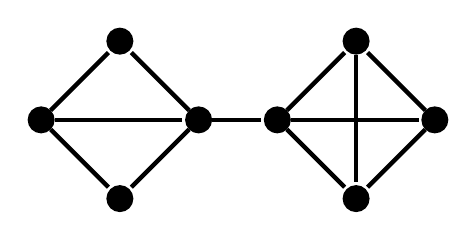
\begin{tikzpicture}[shorten >=1pt, auto, node distance=3cm, ultra thick,main node/.style={circle,fill=black,draw,minimum size=.1cm,inner sep=0pt]}]%
\begin{scope}%[every node/.style={font=\sffamily\Large\bfseries}]%[main node]
\node[main node] (v1) at (0,0) {1};
\node[main node] (v2) at (2,0) {2};
\node[main node] (v3) at (1,1){3};
\node[main node] (v4) at (1,-1){4};
\node[main node] (v5) at (3,0) {5};
\node[main node] (v6) at (5,0) {6};
\node[main node] (v7) at (4,1) {7};
\node[main node] (v8) at (4,-1) {8};
\end{scope}
\begin{scope}[every edge/.style={draw=black,ultra thick}]
\draw  (v1) edge (v2);
\draw  (v1) edge (v3);
\draw  (v1) edge (v4);
\draw  (v2) edge (v3);
\draw  (v2) edge (v4);
\draw  (v2) edge (v5);
\draw  (v5) edge (v6);
\draw  (v5) edge (v7);
\draw  (v5) edge (v8);
\draw  (v6) edge (v7);
\draw  (v6) edge (v8);
\draw  (v7) edge (v8);
\end{scope}
\end{tikzpicture}
\caption*{Graf $G$ posiadający dwie kliki o wielkości 3 oraz klikę wielkości 4, czyli $\omega (G) =4$ }
\end{figure}
\end{description}



\subsection{Programowanie liniowe}
\begin{definition}[Silne twierdzenie dualności]
$$\max _{\bar{x}}f(\bar{x})=\min _{\bar{y}}g(\bar{y})$$
\end{definition}
\begin{problem*}[Znaleźć maksimum funkcji $f$]
\begin{align*}
&f(x_1,x_2,x_3)=6x_1+4x_2+x_3\\
&\left\{\begin{matrix}
3x_1 &+	2x_2 &+	x_3 &\leq 8\\
1x_1 &+	2x_2 &+	x_3 &\leq 5\\
1x_1 &+	0 &		x_3 &\leq 1\\
x_1, &	x_2, &	x_3	&\geq 0
\end{matrix}\right.\\
&\begin{matrix}
y_1:3x_1 &+	2x_2 &+	x_3 &\leq 8\\
y_2:x_1 &+	2x_2 &+ x_3 &\leq 5\\
y_3:x_1 &+		 &  x_3 &\leq 1
\end{matrix}\\
&\text{ZNALEĆ MINIMUM FUNKCJI FUNKCJI }g\\
&\left\{
\begin{matrix}
3y_1	&+ y_2	&+ y_3	&\geq 6\\
2y_1	&+ 2y_2	&& \geq 4\\
y_1		&+ y_2	&+ y_3	&\geq 1\\
y_1,	& y_2,	& y_3	&\geq 0
\end{matrix}
\right.\\
&\max _{x_1x_2x_3} f(x_1,x_2,x_3)\leq \min _{y_1y_2y_3} g(y_1,y_2,y_3)\\
&\text{ dla }y_1=0,\ y_2=2,\ y_3=4\\
&\min _{y_1y_2y_3} g(y_1,y_2,y_3)=14\\
&\text{ dla }x_1=1,\ x_2=2,\ x_3=0\\
&\max _{x_1x_2x_3} f(x_1,x_2,x_3)=14
\end{align*}
\end{problem*}

\begin{problem*}[Znaleźć maksimum funkcji $f$]
\begin{align*}
&f(\bar{x})=\bar{c}^T \bar{x}\\
&\text{przy ograniczeniu: }\\
&A\bar{x}\leq \bar{b}\\
&\bar{x} = \begin{bmatrix}
x_1\\x_2\\x_3
\end{bmatrix} & \bar{c}^T = \begin{bmatrix}
6&4&1
\end{bmatrix}\\
&A=\begin{bmatrix}
3&2&1\\1&2&1\\1&0&1
\end{bmatrix} & \bar{b}=\begin{bmatrix}
8\\5\\1
\end{bmatrix}
\end{align*}
Znaleźć minimum funkcji $g$
$$g(y)=b^Ty$$
przy ograniczeniach
\begin{align*}
&A^T\bar{y}\geq \bar{c}\\
&\bar{y} \geq 0
\end{align*}
\end{problem*}

\begin{theorem}
Jeśli $x^\star$ maksymalizuje po $f(x)$ a $y^\star$ minimalizuje po $g(y)$ wtedy:
$$f(x^\star)=c^Tx^\star =b^Ty^\star =g(y^\star)$$
\end{theorem}

\subsection{Ułamkowe charakterystyki grafów}
\begin{definition}[$\beta (G)$]
Niech $G$ będzie grafem o $n$ wierzchołkach i $m$ krawędziach.\\Niech $\beta (G)$ oznacza wielkość największego skojarzenia w grafie.
\end{definition}

\begin{figure}[H]
\centering
\begin{minipage}{.5\textwidth}
\centering
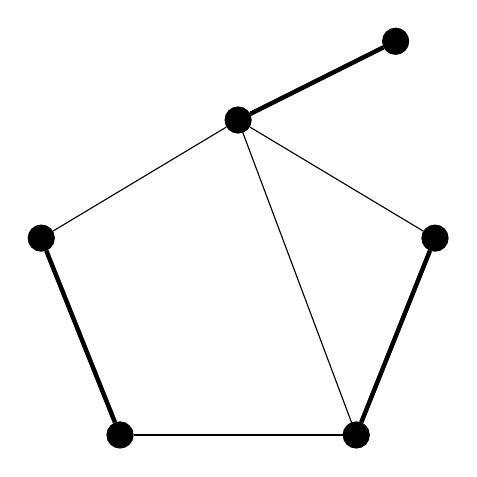
\begin{tikzpicture}[every node/.style={circle, draw, minimum size=0.05cm,fill=black}]
\node (v1) at (2,1) {};
\node (v2) at (0,0) {};
\node (v6) at (-2.5,-1.5) {};
\node (v3) at (2.5,-1.5) {};
\node (v5) at (-1.5,-4) {};
\node (v4) at (1.5,-4) {};
\draw[ultra thick]  (v1) edge (v2);
\draw  (v2) edge (v3);
\draw  (v2) edge (v4);
\draw[ultra thick]  (v3) edge (v4);
\draw  (v4) edge (v5);
\draw[ultra thick]  (v5) edge (v6);
\draw  (v6) edge (v2);
\end{tikzpicture}
\caption*{$\beta (G)=3$, $\gamma (G)=3$}
\end{minipage}%
\begin{minipage}{.5\textwidth}
\centering
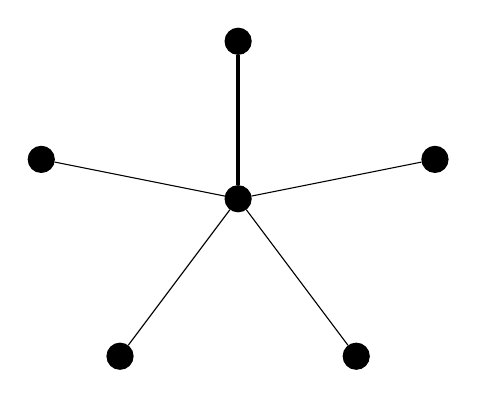
\begin{tikzpicture}[every node/.style={circle, draw, minimum size=0.05cm,fill=black}]
\node (v1) at (0,-2) {};
\node (v2) at (0,0) {};
\node (v6) at (-2.5,-1.5) {};
\node (v3) at (2.5,-1.5) {};
\node (v5) at (-1.5,-4) {};
\node (v4) at (1.5,-4) {};

\draw[ultra thick]  (v2) edge (v1);
\draw  (v1) edge (v3);
\draw  (v4) edge (v1);
\draw  (v1) edge (v5);
\draw  (v6) edge (v1);
\end{tikzpicture}
\caption*{$\beta (G)=1$, $\gamma (G)=1$}
\end{minipage}
\end{figure}

\begin{definition}[$\beta ^\star (G)$]
Dla każdej krawędzi $C\subseteq G$ wprowadzamy zmienną $x_C$ taką, że $x_C=1$ gdy $e$ należy do skojarzenia, a $x_e=0$ gdy nie należy do skojarzenia:
$$f(x_1,\dots x_n)=\sum _{c\in E}x_c$$
($x_c$ $\rightarrow$ wartości na krawędziach) dla każdego wierzchołka $v$ 
$$\forall _v \sum _{v\in e}  x_e \leq 1$$
\begin{align*}
&x_e \in \xcancel{\{0,1\}}\\
&0\leq x_e\leq 1\\
&\beta ^\star (G)\ \rightarrow \text{ułamkowa liczba skojarzenia grafu}
\end{align*}
\end{definition}

\begin{fact}
$$\beta ^\star (G)\geq \beta (G)$$
\end{fact}

Dla każdego wierzchołka wprowadzamy zmienną $y_v$.\\Będziemy szukali minimum następującej funkcji
\begin{align*}
&g(y_1,\dots y_n)=\sum _{v\in V}y_v\\
&\forall _{\begin{matrix}
e\in E\\e\in\{v,w\}
\end{matrix}} y_v+y_w\geq 1\\
&y_v=[0;1]
\end{align*}
\begin{definition}[$\gamma (G)$]
Minimalna liczna pokryciowa $\gamma (G)$, to najmniejsza liczba wierzchołków w zbiorze $w\subseteq V$ takim, że każda krawędź ma przynajmniej jeden koniec w $w$.
\end{definition}

\begin{fact}
$$\gamma (G) \geq \beta (G)$$
\end{fact}
\begin{fact}
$$\gamma (G) \geq \gamma ^\star (G)$$
\end{fact}
\begin{fact}
$$\gamma (G) \geq \gamma ^\star (G)=\beta ^\star (G)\geq \beta (G)$$
\end{fact}

\begin{example*}
przykład:
\begin{figure}[H]
\centering
\begin{minipage}{.5\textwidth}
\centering
\begin{tikzpicture}%[main node/.style={circle, draw, minimum size=0.05cm,fill=black}]
\node (v2) at (0,0) {};
\node (v6) at (-2.5,-1.5) {};
\node (v3) at (2.5,-1.5) {};
\node (v5) at (-1.5,-4) {};
\node (v4) at (1.5,-4) {};
\draw  (v2) edge node[above] {$\sfrac{1}{2}$} (v3);
\draw  (v3) edge node[above] {$\sfrac{1}{2}$} (v4);
\draw  (v4) edge node[above] {$\sfrac{1}{2}$} (v5);
\draw  (v5) edge node[above] {$\sfrac{1}{2}$} (v6);
\draw  (v6) edge node[above] {$\sfrac{1}{2}$} (v2);
\end{tikzpicture}
\caption*{$\beta ^\star (G)\geq 2.5$}
\end{minipage}%
\begin{minipage}{.5\textwidth}
\centering
\begin{tikzpicture}[every node/.style={above,draw}]
\node (v2) at (0,0) {$\sfrac{1}{2}$};
\node (v6) at (-2.5,-1.5) {$\sfrac{1}{2}$};
\node (v3) at (2.5,-1.5) {$\sfrac{1}{2}$};
\node (v5) at (-1.5,-4) {$\sfrac{1}{2}$};
\node (v4) at (1.5,-4) {$\sfrac{1}{2}$};
\draw  (v2) edge (v3);
\draw  (v3) edge (v4);
\draw  (v4) edge (v5);
\draw  (v5) edge (v6);
\draw  (v6) edge (v2);
\end{tikzpicture}
\caption*{$\gamma ^\star (G)\leq 2.5$}
\end{minipage}
\end{figure}
$$\beta ^\star =\gamma ^\star$$
\end{example*}

Oczywiście:
$$\beta (G)\leq \floor{\frac{n}{2}}$$

\textbf{Zadanie:} Uzasadnij, że $$\beta ^\star (G) \leq \frac{n}{2}$$
\begin{proof}
$$\beta ^\star (G)=\gamma ^\star (G) \leq \frac{n}{2}$$
Bo każdemu wierzchołkowi możemy dać wagę $\frac{1}{2}$.
\end{proof}

\begin{figure}[H]
\centering
\begin{minipage}{.5\textwidth}
\centering
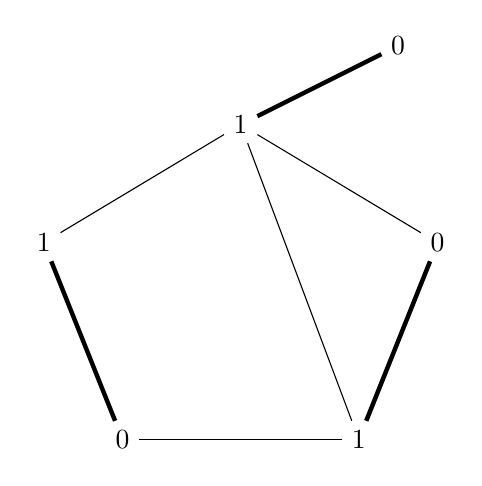
\begin{tikzpicture}%[every node/.style={circle, draw, minimum size=0.05cm,fill=black}]
\node (v1) at (2,1) {0};
\node (v2) at (0,0) {1};
\node (v6) at (-2.5,-1.5) {1};
\node (v3) at (2.5,-1.5) {0};
\node (v5) at (-1.5,-4) {0};
\node (v4) at (1.5,-4) {1};
\draw[ultra thick]  (v1) edge (v2);
\draw  (v2) edge (v3);
\draw  (v2) edge (v4);
\draw[ultra thick]  (v3) edge (v4);
\draw  (v4) edge (v5);
\draw[ultra thick]  (v5) edge (v6);
\draw  (v6) edge (v2);
\end{tikzpicture}
\end{minipage}%
\begin{minipage}{.5\textwidth}
\centering
\begin{tikzpicture}%[every node/.style={circle, draw, minimum size=0.05cm,fill=black}]
\node (v1) at (2,1) {};
\node (v2) at (0,0) {};
\node (v6) at (-2.5,-1.5) {};
\node (v3) at (2.5,-1.5) {};
\node (v5) at (-1.5,-4) {};
\node (v4) at (1.5,-4) {};
\draw  (v1) edge node[above] {1} (v2);
\draw  (v2) edge node[above] {0} (v3);
\draw  (v2) edge node[above] {1} (v4);
\draw  (v3) edge node[above] {1} (v4);
\draw  (v4) edge node[above] {0} (v5);
\draw  (v5) edge node[above] {1} (v6);
\draw  (v6) edge node[above] {0} (v2);
\end{tikzpicture}
\end{minipage}
\end{figure}

\begin{theorem}[D. Konig 1931]
Dla grafów dwudzielnych:
$$\begin{array}{ccc}
\beta (G) & = & \gamma (G) \\
\parallel &   & \parallel \\
\beta ^\star (G) & = & \gamma ^\star (G)
\end{array}$$
\end{theorem}

\begin{definition}[$\omega ^\star (G)$]
Ułamkową liczbą klikową $\omega ^\star (G)$ nazywamy maksymalną wartość funkcji:
$$f(x_1,\dots x_n)=\sum _{v\in V} x_v$$ 
przy czym dla każdego zbioru niezależnego $I$
\begin{align*}
&\sum _{v\in I} x_v\\
&x_v\geq 0\ \ x_v\in \{0,1\}
\end{align*}
\end{definition}

\begin{definition}[Ułamkowa liczba chromatyczna $\chi ^\star (G)$]
Każdemu zbiorowi niezależnemu $I$ przyporządkowujemy zmienną losową $y_I$ i minimalizujemy: $$\sum _I y_I$$ przy ograniczeniu, że 
\begin{align*}
&\forall _{v\in V} \sum _{\{I:v\in I\}}y_I\geq 1\\
&y_I\geq 0\\
&\text{dla }\chi (G) \text{ będzie } y_I=\{0,1\}
\end{align*}
\end{definition}

\begin{fact}
$$\chi (G)\geq \chi ^\star(G)=\omega ^\star(G)\geq \omega (G)$$
\end{fact}

\begin{figure}[H]
\centering
\begin{tikzpicture}%[main node/.style={circle, draw, minimum size=0.05cm,fill=black}]
\node (v2) at (0,0) {$v_1$};
\node (v6) at (-2.5,-1.5) {$v_5$};
\node (v3) at (2.5,-1.5) {$v_2$};
\node (v5) at (-1.5,-4) {$v_4$};
\node (v4) at (1.5,-4) {$v_3$};
\draw  (v2) edge (v3);
\draw  (v3) edge (v4);
\draw  (v4) edge (v5);
\draw  (v5) edge (v6);
\draw  (v6) edge (v2);
\end{tikzpicture}
\end{figure}
\begin{align*}
&v_1=v_2=v_3=v_4=v_5=\frac{1}{2}\\
&\text{zbiory niezależne: } 
\underset{\sfrac{1}{2}}{\{v_1,v_3\}}, \underset{\sfrac{1}{2}}{\{v_2,v_4\}},
\underset{\sfrac{1}{2}}{\{v_3,v_5\}}, \underset{\sfrac{1}{2}}{\{v_4,v_1\}},
\underset{\sfrac{1}{2}}{\{v_5,v_2\}}\\
&\chi (G)=3 & \omega (G) = 2\\
&\chi ^\star(G)\leq \sfrac{5}{2} & \omega ^\star(G)\geq \sfrac{5}{2}\\
&\chi ^\star(G) = \omega ^\star(G)= \sfrac{5}{2}\\
&\text{Ta własność } \chi (G)=\omega (G) \text{ jest bardzo rzadka wśród grafów}
\end{align*}





